并行内核的第二种形式是在执行范围内执行,其中工作项属于工作组,符合想在内核中表达局域性的概念。不同类型的工作组定义和保证了不同的行为,使我们能够了解和/或控制将工作映射到特定的硬件平台。\par

显式的ND-range内核是规范的并行——我们对每种工作组的工作进行映射,并且实现必须遵守这种映射。但是,这并不是完全定死的,因为工作组本身可以按任何顺序执行,并且实现将每种类型工作组映射到硬件资源上保留一定的自由度。这种说明性和描述性编程的结合使我们能进行局部性设计和调优内核,而不会影响可移植性。\par

与数据并行内核一样,ND-range内核以SPMD风格编写,其中所有工作项执行应用于多个数据块的相同内核。关键的区别是,每个程序实例可以查询在工作组中的位置,并可以访问特定于每种类型组的其他功能。\par

\hspace*{\fill} \par %插入空行
\textbf{理解ND-Range并行内核}

ND-Range内核的执行范围可以划分为工作组、子工作组和工作项。ND-range表示总的执行范围,将其划分为统一大小的工作组(即工作组大小必须在每个维度上精确划分ND-range大小)。每个工作组可以通过实现进一步划分为子组。工作项和每种类型的组定义的执行模型是编写正确和可移植程序的重要部分。\par

图4-12展示了一个将(8,8,8)的ND-range划分为8个大小(4,4,4)的工作组的例子。每个工作组包含由4个工作项组成的16个一维子工作组。注意维度的编号:子工作组是一维的,因此ND-range和工作组的维度2,变成子组的维度0。\par

\hspace*{\fill} \par %插入空行
图4-12 3维ND-range划分为工作组、子工作组和工作项
\begin{center}
	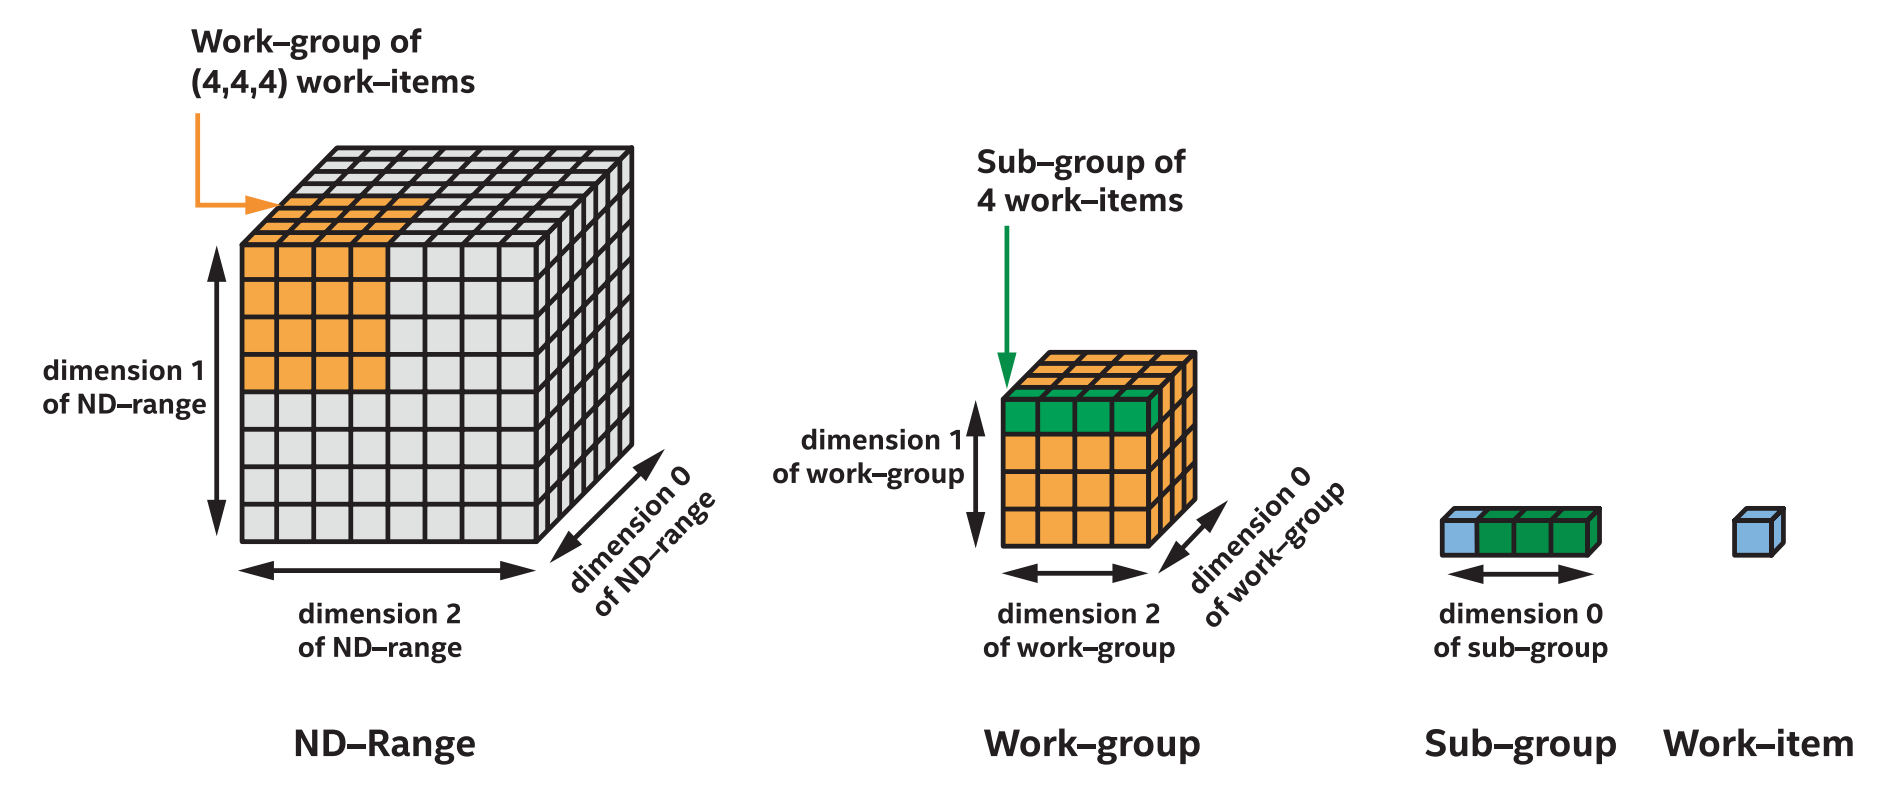
\includegraphics[width=1.\textwidth]{content/chapter-4/images/5}
\end{center}

每种类型的组到硬件资源的映射由实现定义,这种灵活性使程序能够在各种各样的硬件上执行。例如,工作项可以完全顺序执行,可以由硬件线程和/或SIMD指令并行执行,甚至可以由特定内核配置的硬件执行。\par

本章中,我们只关注在通用平台上ND-range执行模型的语义,并且不讨论对任何一个平台的映射。关于GPU、CPU和FPGA的硬件映射和性能建议,分别在第15、16和17章再进介绍。\par

\hspace*{\fill} \par %插入空行
\textbf{工作项}

工作项表示内核函数的各个实例。在没有其他分组的情况下,工作项可以以任何顺序执行,并且不能相互通信或同步,除非通过对全局内存的原子内存操作(参见第19章)。\par

\hspace*{\fill} \par %插入空行
\textbf{工作组}

ND-Range中的工作项可以组织成工作组。工作组可以以任何顺序执行,并且不同工作组中的工作项不能相互通信,除非通过对全局内存的原子内存操作(参见第19章)。然而,当使用某些构造时,一个工作组中的工作项具有并发调度保证,并且这种局部性提供了额外的能力:\par

\begin{enumerate}
	\item 工作组中的工作项可以访问工作组本地内存,这些内存可以映射到某些设备上的专用快速内存(参见第9章)。
	\item 工作组中的工作项可以使用工作组栅栏进行同步,并使用工作组内存栅栏保证内存一致性(参见第9章)。
	\item 工作组中的工作项可以访问组函数,提供可通信例程的实现(见第9章)和常规并行模式(如归约和扫描)(见第14章)。
\end{enumerate}

工作组中的工作项数量通常是在运行时为内核配置的,最佳分组将取决于可用的并行度(即ND-Range的大小)和目标设备的属性。我们可以使用设备类的查询函数,来确定特定设备支持的每个工作组的最大工作项数(见第12章),我们的责任是确保每个内核请求的工作组大小是有效的。\par

首先,工作组中的工作项可以调度单个计算单元,但工作组的数量和计算单元的数量之间不需要有任何关系。ND-Range内的工作组数量可能比给定设备可并发执行的工作组数量大很多倍!我们可能会依靠特定于设备的调度,尝试和编写内核同步工作组,但我们强烈建议不要这样做,因为不能保证与实现可能会在一个与之前不同的设备上运行。\par

其次,工作组中的工作项可以同时安排工作,但不能保证工作的独立性时——在工作组中使用栅栏和集合,可以对组内工作项进行同步。同一个工作组中工作项之间的通信和同步,只有在使用栅栏和集合操作时才能保证安全,手工编码的同步可能会造成死锁。\par

\begin{tcolorbox}[colback=blue!5!white,colframe=blue!75!black, title=对于工作组的思考]
工作组在许多方面与其他编程模型中的任务概念相似(例如:线程块):任务可以按任何顺序执行(由调度程序控制);在机器上开辟大量的任务是可能的(甚至是可取的);尝试在一组任务之间使用栅栏,通常不是一个好主意(因为它可能非常昂贵或与调度器不兼容)。如果已经熟悉了基于任务的编程模型,那么会发现将工作组看作是数据并行的任务就好理解了。
\end{tcolorbox}

\hspace*{\fill} \par %插入空行
\textbf{子工作组}

许多硬件平台上,工作组中的子工作组在执行时具有调度上的保证。例如,子工作组中的工作项可以同时执行,因为可以映射到独立的硬件线程,子工作组本身可以在保证内核进度的情况下执行。\par

使用单一平台时,很容易在代码中加入执行模型的假设,但这使得内核不安全且不可移植——当在不同的编译器之间移植时,甚至当在来自同一厂商的不同一代硬件之间迁移时,都可能会崩溃!\par

将子工作组定义为语言的核心部分,为我们提供了一种安全的选择。利用子工作组功能还允许我们在底层硬件上执行工作项,并且这还可以为跨平台实现高性能级别的应用。\par

与工作组一样,子工作组中的工作项可以同步、保证内存一致性,或通过工作组功能执行常见的并行模式。但是,对于子工作组没有等价的工作组本地内存(也就是说,没有子组本地内存)。相反,子工作组中的工作项可以直接交换数据——无需显式的内存操作——使用shuffle操作(第9章)。\par

子工作组的某些功能由实现定义,不在我们的控制范围内。但对于给定的设备、内核和ND-Range组合,子工作组具有固定的(一维的)大小,可以使用内核类的查询函数来查询这个大小(见第10章)。默认情况下,每个子工作组的工作项数量也由实现选择——可以通过在编译时请求特定的子组大小来覆盖这个行为,但是必须确保请求的子工作组大小与设备兼容。\par

与工作组类似,子工作组中的工作项只保证并行执行——实现可以自由地顺序执行子工作组中的每个工作项,并且只有在遇到子工作组的集合功能时才会在工作项之间切换。子工作组的特殊之处在于,某些设备保证独立地执行——工作组中的所有子工作组都保证最终执行(取得进展),这是若干生产者-消费者模式的基石。这个独立的执行是否能保持,可以通过设备查询来确定。\par

\begin{tcolorbox}[colback=blue!5!white,colframe=blue!75!black, title=对于子工作组的思考]
如果考虑显式向量化的编程模型,那么将每个子工作组看作打包到SIMD寄存器中的一组工作项可能会更容易理解,其中子工作组中的每个工作项对应于一个SIMD通道。当多个子工作组同时执行时,硬件设备可以保证任务的执行,这种模型扩展会把每个子工作组当作并行执行的独立向量指令流来对待。
\end{tcolorbox}

\hspace*{\fill} \par %插入空行
图4-13 用ND-range parallel\_for表示矩阵乘法
\begin{lstlisting}[caption={}]
range global{N, N};
range local{B, B};
h.parallel_for(nd_range{global, local}, [=](nd_item<2> it) {
	int j = it.get_global_id(0);
	int i = it.get_global_id(1);
	
	for (int k = 0; k < N; ++k)
		c[j][i] += a[j][k] * b[k][i];
});
\end{lstlisting}

\hspace*{\fill} \par %插入空行
\textbf{编写ND-Range数据并行内核}

图4-13重新实现了使用ND-range parallel\_for内核编写的矩阵乘法内核,图4-14中展示了这个内核是如何映射到每个工作项中的。以这种方式对工作项进行分组,从而保证本地的访问高效性,提高缓存命中率:例如,工作组在图4-14的大小是(4,4),包含16个工作项,为了每个工作项都能执行正常,相应的数据需要加载四次。\par

\hspace*{\fill} \par %插入空行
图4-14 将矩阵乘法映射到工作组和工作项
\begin{center}
	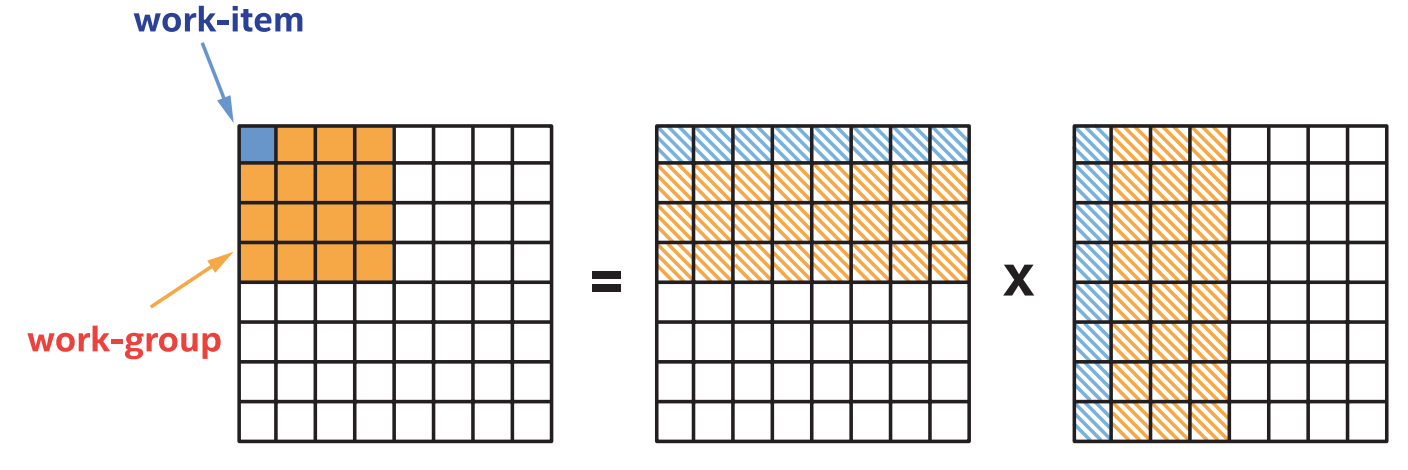
\includegraphics[width=1.\textwidth]{content/chapter-4/images/8}
\end{center}

目前为止,矩阵乘法示例依赖于硬件缓存对同一个工作组中工作项的A和B矩阵的重复访问进行优化。这样的硬件缓存在传统的CPU架构中很常见,而且在GPU架构中也越来越常见,但是也有其他架构(如上一代GPU、fpga)带有显式管理的“暂存”内存。ND-range内核可以使用本地访问器来说明工作组的本地内存分配的位置,然后实现就可以自由地将这些分配映射到特定的内存(它存在的地方)。工作组本地内存的使用将在第9章中介绍。\par

\hspace*{\fill} \par %插入空行
\textbf{ND-Range数据并行内核的细节}

与数据并行内核相比,ND-Range内核可以使用不同的类:nd\_range替换range,nd\_item替换item。还有两个新类,表示工作项属于的不同类型的组:绑定工作组的功能封装在group类中,绑定到子工作组的功能封装在sub\_group类中。\par

\hspace*{\fill} \par %插入空行
\textbf{nd\_range类}

nd\_range表示使用range类的两个实例组成的执行范围:一个表示全局执行范围,另一个表示每个工作组的本地执行范围。图4-15给出了nd\_range类的简化定义。\par

nd\_range类根本没有提到子工作组,这有点令人惊讶:子工作组范围在构造期间没有指定,不能查询。这有两个原因,1.子工作组是可以忽略的底层实现细节。2.有设备只支持固定的的子工作组大小,从而指定大小没有必要。所有与子工作组相关的功能都封装在一个特定的类中,稍后将对此再进行讨论。\par

\hspace*{\fill} \par %插入空行
图4-15 简化定义的nd\_range类
\begin{lstlisting}[caption={}]
template <int Dimensions = 1>
class nd_range {
public:
	// Construct an nd_range from global and work-group local ranges
	nd_range(range<Dimensions> global, range<Dimensions> local);
	
	// Return the global and work-group local ranges
	range<Dimensions> get_global_range() const;
	range<Dimensions> get_local_range() const;
	
	// Return the number of work-groups in the global range
	range<Dimensions> get_group_range() const;
};
\end{lstlisting}

\hspace*{\fill} \par %插入空行
\textbf{nd\_item类}

nd\_item是工作项的ND-Range形式,同样封装了内核的执行范围和工作项在该范围内的索引。nd\_item与item的区别在于范围中的位置查询和表示,如图4-16中简化的类定义所示。\par

例如,可以使用get\_global\_id()函数在(全局)ND-Range中查询工作项的索引,或者使用get\_local\_id()函数在(本地)父工作组中查询工作项的索引。\par

nd\_item类还提供了获取描述项所属的工作组和子工作组的类句柄的函数。这些类为查询DN-Range的项目索引提供了另一种方式。我们强烈推荐使用这些类来编写内核,而不是依赖于nd\_item:使用group和sub\_group类通常更简洁,更清晰,也更符合DPC++的未来方向。\par

\hspace*{\fill} \par %插入空行
图4-16 简化定义的nd\_item类
\begin{lstlisting}[caption={}]
template <int Dimensions = 1>
class nd_item {
public:
	// Return the index of this item in the kernel's execution range
	id<Dimensions> get_global_id() const;
	size_t get_global_id(int dimension) const;
	size_t get_global_linear_id() const;
	
	// Return the execution range of the kernel executed by this item
	range<Dimensions> get_global_range() const;
	size_t get_global_range(int dimension) const;
	
	// Return the index of this item within its parent work-group
	id<Dimensions> get_local_id() const;
	size_t get_local_id(int dimension) const;
	size_t get_local_linear_id() const;
	
	// Return the execution range of this item's parent work-group
	range<Dimensions> get_local_range() const;
	size_t get_local_range(int dimension) const;
	
	// Return a handle to the work-group
	// or sub-group containing this item
	group<Dimensions> get_group() const;
	sub_group get_sub_group() const;
};
\end{lstlisting}

\hspace*{\fill} \par %插入空行
\textbf{group类}

group类封装了与工作组相关的所有功能,简化的定义如图4-17所示。\par

\hspace*{\fill} \par %插入空行
图4-17 简化定义的group类
\begin{lstlisting}[caption={}]
template <int Dimensions = 1>
class group {
public:
	// Return the index of this group in the kernel's execution range
	id<Dimensions> get_id() const;
	size_t get_id(int dimension) const;
	size_t get_linear_id() const;
	
	// Return the number of groups in the kernel's execution range
	range<Dimensions> get_group_range() const;
	size_t get_group_range(int dimension) const;
	
	// Return the number of work-items in this group
	range<Dimensions> get_local_range() const;
	size_t get_local_range(int dimension) const;
};
\end{lstlisting}

group类提供的许多函数在nd\_item类中都有等价的函数:例如,调用group.get\_id()等价于调用item.get\_group\_id(),然后调用group。Get \_local\_range()等价于调用item.get\_local\_range()。如果不使用该类的任何工作组函数,还应该使用它吗?直接使用nd\_item中的函数,不是更简单吗?这里有一个折衷的方式:使用group要求我们编写更多的代码,但这些代码可能更容易阅读。例如,图4-18中的代码片段:body由工作组中的所有工作项调用,parallel\_for的中的get\_local\_range()返回的范围就是工作组的范围。只用nd\_item就可以很容易地编写相同的代码,但可能很难理解。\par

\hspace*{\fill} \par %插入空行
图4-18 使用group类来提高可读性
\begin{lstlisting}[caption={}]
void body(group& g);
h.parallel_for(nd_range{global, local}, [=](nd_item<1> it) {
	group<1> g = it.get_group();
	range<1> r = g.get_local_range();
	...
	body(g);
});
\end{lstlisting}

\hspace*{\fill} \par %插入空行
\textbf{sub\_group类}

sub\_group类封装了与子工作组相关的功能,简化的定义如图4-19所示。与工作组不同,sub\_group类是访问子工作组功能的唯一方法,其函数在nd\_item中没有重复。sub\_group类中的查询都是相对于调用工作项进行解释的:例如,get\_local\_id()返回子组中调用工作项的本地索引。\par

\hspace*{\fill} \par %插入空行
图4-19 简化定义的sub\_group类
\begin{lstlisting}[caption={}]
class sub_group {
	public:
	// Return the index of the sub-group
	id<1> get_group_id() const;
	
	// Return the number of sub-groups in this item's parent work-group
	range<1> get_group_range() const;
	
	// Return the index of the work-item in this sub-group
	id<1> get_local_id() const;
	
	// Return the number of work-items in this sub-group
	range<1> get_local_range() const;
	
	// Return the maximum number of work-items in any 
	// sub-group in this item's parent work-group
	range<1> get_max_local_range() const;
};
\end{lstlisting}

有一些功能用于查询当前子工作组中的工作项数量,以及工作组中任何子工作组中的最大的工作项数量。这些方式取决于特定设备对于子工作组的实现的方式,但其目的是反映编译器目标子工作组大小和运行时子工作组大小之间的差异。例如,非常小的工作组可能包含比编译时子工作组更少的工作项,或者不同大小的子工作组可能用于处理不能被子组大小整除的工作组。\par





